\documentclass[a4paper]{article}

\usepackage[utf8]{inputenc}
\usepackage[T1]{fontenc}
\usepackage{textcomp}
\usepackage{listings}
\usepackage{lmodern}
\usepackage{amsfonts}
\usepackage{titling}
\usepackage{lipsum}
\usepackage[left=1in, right=1in, bottom=1in, top=1in]{geometry}
\usepackage{amsthm}
\usepackage{tcolorbox}
\usepackage{hyperref}
\usepackage{xcolor}
\usepackage{graphicx}
\usepackage{makeidx}
\usepackage{tikz}
\usepackage{cases}
\usepackage{apacite}
\usepackage{tkz-berge}
\usepackage{url}
\usepackage{tgtermes}
\usepackage{sectsty}
\usepackage{subcaption}
\usepackage{setspace}
\usepackage{float}
\usepackage{amsmath, amssymb}


% figure support
\usepackage{import}
\usepackage{xifthen}
\pdfminorversion=7
\usepackage{pdfpages}
\usepackage{transparent}
\usepackage{color}
\newcommand{\incfig}[2][1]{%
    \def\svgwidth{#1\columnwidth}
    \import{./figures/}{#2.pdf_tex}
}

%mathstyling
\theoremstyle{plain}
\newtheorem{thm}{Theorem}[section]
\newtheorem{lem}[thm]{Lemma}
\newtheorem{prop}[thm]{Proposition}
\newtheorem*{cor}{Corollary}

\theoremstyle{definition}
\newtheorem{defn}{Definition}[section]
\newtheorem{conj}{Conjecture}[section]
\newtheorem{exmp}{Example}[section]
\newtheorem{axiom}{Axiom}
\theoremstyle{remark}
\newtheorem*{rem}{Remark}
\newtheorem*{note}{Note}

\definecolor{darkgreen}{rgb}{0.0, 0.5, 0.0}

\pdfsuppresswarningpagegroup=1
\lstset{
tabsize = 4, %% set tab space width
showstringspaces = false, %% prevent space marking in strings, string is defined as the text that is generally printed directly to the console
numbers = left, %% display line numbers on the left
commentstyle = \color{darkgreen}, %% set comment color
keywordstyle = \color{blue}, %% set keyword color
stringstyle = \color{red}, %% set string color
rulecolor = \color{black}, %% set frame color to avoid being affected by text color
basicstyle = \small \ttfamily , %% set listing font and size
breaklines = true, %% enable line breaking
numberstyle = \tiny,
  frame=none,
  xleftmargin=2pt,
  stepnumber=1,
  belowcaptionskip=\bigskipamount,
  captionpos=b,
  escapeinside={*'}{'*},
  language=haskell,
  tabsize=2,
  emphstyle={\bf},
  showspaces=false,
  columns=flexible,
  showstringspaces=false,
  morecomment=[l]\%,
}
\begin{document}
	\begin{titlepage}
	\begin{center}
	\large
	University of Warwick \\
	Department of Computer Science \\
	\huge
	\vspace{50mm}
	\rule{\linewidth}{0.5pt} \\
	CS263 \\
	\vspace{5mm}
	\Large
	Cyber Security
	\rule{\linewidth}{0.5pt}
	\vspace{5mm}
	\begin{figure}[H]
	\centering
	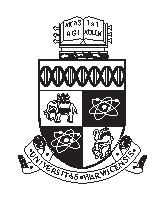
\includegraphics[width=0.4\textwidth]{crest_black.eps}
	\end{figure}
	\vspace{37mm}
	Cem Yilmaz \\
	\today
	\end{center}
	\end{titlepage}
	\tableofcontents
	\newpage
	\section{History Cyber Security}
	\begin{tcolorbox}[colback=black!3!white,colframe=black!60!white,title=\begin{defn}Cybersecurity \label{Cybersecurity}\end{defn}]
	Cyber security is the application of technologies, processes, and controls to protect systems, networks, programs, devices and data from cyber attacks
	\end{tcolorbox}
	\subsection{1940-1950}
	The first digital computer was creating during World War II. Work on Electronic Numerical Integrator and Computer (ENIAC) began in 1943 and was completed in 1945. It was designed specifically for computing values for artillery range tables. It occupied a 15 by 9 metre room. Threats were nearly non-existent and in 1949 John Von Neumann speculated the existence of computer viruses.  \\
	In the 1950s hacking telephones has emerged, which was a precursor to hacking computers. Phone phreaks hijacked telephone protocols that allowed engineers to work on telecom networks remotely. They used a Blue Box to make free long-distance calls. In short term, the Bell Telephone Company took legal actions against offenders. Phreaking largely ended in 1983 when the company upgraded its telephone lines. 
	\subsection{1960-1970}
	1960 was the birth of ethical hacking. Mainframes were locked in secure rooms and in 1967 IBM invited students to try out their computer. They were able to gain access to different parts of the system. Companies realised the importance of developing security measures to keep hackers out. \\
	1970s the advanced research projects network (ARPANET), a precursor to the internet was developed. The network was operation in 1971 and birthed the mark of cyber security. In 1971, Bob Thomas created a Creeper, a computer program that moved across ARPANET's network. Ray Tomlinson modified Creeper to copy itself between computers. This was the first example of a computer worm. In 1972, Tomlinson wrote Reaper to chase and delete Creeper. Reaper was the first anti-virus program.
	\subsection{1980-1990}
	In 1983, the US department of defense published the Trusted Computer System Evaluation Criteria, known as the Orange Book. This standard set basic requirements to assess the effectiveness of computer security controls built into a computer system. In 1987, the first commercial anti viruses were developed. In 1988, the Morris worm resulted in denial of service attack, affecting thousands of Unix machines connected to the internet. He was the first one to be charged under the 1986 Computer Fraud and Abuse Act. This event led the Defense Advanced Research Project Agency (DARPA) to fund the establishment of the Coordination Center of the Computer Emergency Response Team. \\
	In the 1990s a new type of viruses were developed. In 1991 appeared the first polymorphic values. Chameleon infected all .com files in the same directory. In 1999, David Lee Smith released the Melissa macro virus. The cost of cleaning up infected systems was estimated to 80 million USD. To keep communication private between a client a server, Netscape developed the SSL protocol in 1994. 
	\subsection{21st Century}
	With the growth of the internet, the scape and type of attacks changed. Internet Relay Chat systems were infected by worms. Use of fileless attacks (viruses that disguise themselves as legitimate software) to compromise computer systems were done. Operation Cobalt Kitty used a fileless attack to target a global corporation in Asia. Zero-day attacks that targeted Internet-of-Things devices. The NSO Group also developed Pegasus malware and is selling to governments. It was discovered in 2016 and targets Android and IOS devices. It is able to spy on users through a zero-click exploit. As a result, standards and regulations were released. SP 1271 provides a starting guide for a framework that you may download.
	\section{Cybersecurity and cybercrime}
	\subsection{Cybercrime}
	
	Examples of cybercrimes:
	\begin{itemize}
		\item Theft of financial data
		\item illegal gambling
		\item cyberespionage e.g., accessing  a company/government system
		\item cryptojacking
		\item ransomware attack
	\end{itemize}
	\subsection{Cybersecurity Principles}
	Some principles are the CIA triad: confidentiality, integrity, availability. Defensive measures, applied to prevent, detect and mitigate threats and security vulnerabilities. Testing is also important, as defensive measures need to be regularly tested and scanned for vulnerabilities. This is called penetration testing. We can test employees using phishing emails. Training is also important, which involves training IT team and employees. Response is also a must and requires a ready-to-deploy response plan in case of a security incident to ensure business continuity and mitigate a threat. The treats include
	\begin{itemize}
		\item Destruction
		\item Modification
		\item Theft
		\item Disclosure
		\item Interruption
	\end{itemize}
	Examples of cyber threats and exploit are
	\begin{itemize}
		\item Buffer overflow - an exploit where a program attempts to put more data in a buffer than it can hold. Writing outside the bounds of a block of allocated memory can corrupt data, crash the product or cause the execution of malicious code.
		\item Man in the middle attack - an attacker intercepts and relays a message between two parties
		\item Denial of Service attack - an attacker prevents authorised users from accessing a service
		\item Zero-day exploit - a vulnerability in a system that has been discovered by an attacker before the vendor is aware of it
		\item Backdoor - method of bypassing normal authentication and gaining unauthorised access to a system or application
		\item Trojan horse - a program with an overt purpose and a malicious covert one.
	\end{itemize}
	Furthermore, types of cyber criminals are the following:
	\begin{itemize}
		\item Script kiddie - use existing software or scripts to launch attacks on computers and networks
		\item Scammers - they use deceptive schemes e.g., email, phone calls to trick their victims
		\item Insider Threats - could be caused by an ex-employee who still has access to a company's computing system.
		\item Hacktivists - they carry out cyberattacks based on a shared ideology
		\item Cybercrime groups - they work together anonymously to build tools for hacking
		\item State actors - backed by a government to forcefully target another government, individual or organisation. 
	\end{itemize}
\subsection{Internet Data}
The International Data Corporation (IDC) predicts that global data sphere will grow from 33 Zettabytes in 2018 to 175 zettabytes in 2025. One zettabyte is equal to $10^{21}$. About $50\%$ of the ata will reside in cloud in 2025. Google processes 8.5 billion searches per day. As of May 2021, one can buy on the dark web a
\begin{itemize}
	\item Hacked facebook account for $65$
	\item Hacked and verified coinbase account for $610$ 
	\item Complete health record for $250$ 
	\item Cloned visa with PIN for $25$ 
	\item Hacked Gmail account for $80$
\end{itemize}
All prices are listed in USD. DOMO is a cloud-based company that specialises in business intelligence tools and data visualisation. The average worldwide cost is $4.35$ million for a data breach. 
\subsection{Threats and Malware}
Top targeted industries are education, healthcare and government. Top malware types used are Adware, phishing and finally botnet. 
\begin{tcolorbox}[colback=black!3!white,colframe=black!60!white,title=\begin{defn}Adware \label{Adware}\end{defn}]
Software that displays unwanted pop-up advertisements which can appear on your computer or mobile device.
\end{tcolorbox}
\begin{tcolorbox}[colback=black!3!white,colframe=black!60!white,title=\begin{defn}Phishing \label{Phishing}\end{defn}]
Phishing is a type of social engineering attack. An attacker, masquerading as a trusted entity, tricks a victim into opening an email, instant message, or text message. It aims to steal user data. Some examples include, but are not limited to email phishing, whaling, smishing and vishing, angler phishing
\end{tcolorbox}
	\begin{tcolorbox}[colback=black!3!white,colframe=black!60!white,title=\begin{defn}Botnets \label{Botnets}\end{defn}]
	Botnet are networks of hijacked computers. Botnet is formed from the words Bot and Network. They are used to launch Distributed Denial of Service attacks, phishing attacks and cryptojacking. Malicious actors control a Botnet via a command and control server. To protect against Botnets, technical controls would include AV software, Intrusion detection system (IDS), Intrusion prevention system (IPS). Security policies and training people can also help prevent botnets from emerging.
	\end{tcolorbox}
	
\end{document}
